\setcounter{secnumdepth}{0} 
\subsection{Summary}

% Our oceans host enormous species richness, provide multiple ecosystem
% services, sustain vibrant economies, and play a critical role in
% climate regulation.  Yet the health of these rich live bodies  that
% society greatly depends on, has been significantly threatened by
% long-standing unsustainable human activities and a globally changing
% climate.

The oceans make this planet habitable and provide a variety of
essential ecosystem services ranging from climate regulation through
control of greenhouse gases to provisioning about 17\% of protein
consumed by humans.  The oceans are changing as a consequence of human
activity and yet because our knowledge about this ecosystem is
limited, we cannot accurately model and predict how it will behave in
the future.  The oceans are vast, occupying almost 71\% of our
planet’s surface and yet less than 10\% of it has been studied.  This
system is severely under sampled and despite breathtaking advances in
observational technology, robotics, and computer science, we have not
addressed the mismatch in the scales of observation needed and our
traditional ways of studying the ocean.
% This system is severely under sampled and despite breathtaking
% advances in observational technology, robotics, and computer
% science, our ways of studying the oceans in-situ have not changed
% much over the last few hundred years.
The absence of a reliable, efficient and timely monitoring system for
ocean health is greatly impeding our capacity to respond to and
prevent human-induced threats in a timely, context-relevant and
effective way.

This is especially important in coastal regions because these areas
mediate most of the interactions between a significant percentage of
the world population and the oceans.  In addition to other global
pressures, urban population growth has exacerbated pressures on
coastal ecosystems resulting in unhealthy alterations (e.g., toxic
algal blooms, oxygen depletion also referred to as hypoxia) and
deleterious effects on fisheries and human health. These problems are
likely to accelerate in the coming decades as extreme weather events
and storm surges will likely enhance agricultural pollution runoff and
coastal erosion, leading to a worsening coastal water quality.

We urgently need a reliable, efficient, and affordable data-gathering,
assimilating and ocean modeling capability to help us monitor,
understand, and effectively manage the key ocean processes that are
essential to ocean health and negatively impacted by human
activity. Based on our team's combined knowledge and experience in
this field, we believe that an integrative ocean-management approach,
and the protection of our ocean capital can only be achieved with the
help of coordinated observations from space, and aerial, surface and
underwater robots guided by Artificial Intelligence (AI). We are
proposing this innovative and first-of-its-kind (hardware and
software) solution by building a portable robotic observatory that can
be rapidly deployed anywhere in the world for observing, analyzing and
evaluating the health of our endangered coastal waters
(Fig. \ref{fig:mega-cities}).

% Our oceans host enormous biodiversity, provide multiple ecosystem
% services, sustain vibrant economies, and play a significant role in
% climate regulation, but are threatened by human activity and climate
% change.  We need a \textbf{sustained}, \textbf{persistent}, and
% \textbf{affordable} data gathering and assimilating capability to help
% us understand and monitor how key processes such as acidification,
% hypoxia, toxic blooms, pollution and erosion (amongst others) are
% impacting global ocean sustainability and stewardship.  In coastal
% regions, this is especially important, because these areas mediate
% most of the interactions between a significant percentage of the world
% population and the oceans.

% Urban population growth has exacerbated the pressures on the coastal
% ecosystem.  For example, resultant toxic blooms and oxygen depletion
% have had deleterious effects on fisheries and other critical resources
% that coastal populations depend on, while also impacting human
% health. Furthermore, extreme weather events induced by climate change
% will only hasten the worsening of water quality in these areas because
% of enhanced runoff, coastal erosion and storm surges. An integrative
% sea management approach and the protection of natural capital and
% marine ecosystem resources can only be achieved with the help of
% coordinated observations from space, aerial, surface and underwater
% robots guided by Artificial Intelligence (AI).
% % while providing continual and reliable oceanographic data.

% Many large telescopes point toward the heavens, but no such
% observational system exists for looking at and into our oceans and
% yet, the ocean is the primary driver for much of the planet's weather.
% Our mission is to build a portable, robotic observatory for observing,
% analyzing and managing the health of our endangered coastal waters
% which can be rapidly deployed anywhere in the world
% (Fig. \ref{fig:mega-cities}).


% robotic technologies reduces
% deployment time to provide opportune solutions and consequently,
% leverages the latest techniques in AI, Robotics and software
% engineering.


% It
% will provide information for water quality measurements suitable for
% lay persons who can obtain and interpret near real-time (hours) data
% visualized at spatial and temporal scales to provide actionable
% information to deal with coastal pollution, erosion, toxic waters and
% sediment laden plumes.

\subsection{The Idea}


% \begin{wrapfigure}{r}{3.8in} %{2.1in - .75\columnsep}
%   % \vspace{-\intextsep}
%     \hspace*{-.35\columnsep}
% \end{wrapfigure}

\pro (Movable ocEan roboTic obsErvatORy) is conceived as a modular
system with bespoke approaches related to water quality in the world’s
coastal zones.  The system constitutes both a vertical integration of
state-of-the-art hardware including a small satellite (\smle)
constellation, as well as in-situ air, surface and underwater
vehicles, with innovative software to control and visualize the
information gathered, as well as horizontal integration across
disciplines of computer science, marine robotics, engineering, ocean
modeling and oceanography. The frequent revisit times over a region
that only a constellation of \smle s can provide, coupled with the
latest smart and adaptive AI techniques, will enable robots to deliver
systematic and opportune observations of parameters relevant to
coastal water quality and ocean processes in near real-time
(Fig. \ref{fig:mega-cities}).

% \pro (A Portable Robotic Observatory for Coordinated Oceanographic
% Observations) will be a modular system with bespoke approaches related
% to water quality in the world's coastal zones with mega-cities. It
% will integrate state-of-the-art hardware (including a small satellite
% (\smle) constellation, in-situ air, surface and underwater vehicles)
% with innovative software to control and visualize the information
% gathered. With frequent revisit times over a region -- only possible
% with the use of a constellation of \smle's -- coupled with latest smart
% and adaptive AI techniques, robots can provide systematic and
% opportune observations in near real-time.

% ****************************
% Using \proe, stakeholders across governments, industry, science,
% nonprofits and citizenry will make use of layered views ranging from
% basic visuals to the complex queries needed for effective management
% of resources and increased scientific knowledge.  Ocean models in the
% cloud, will integrate the information collected from multiple
% platforms, robotic vehicles as well as satellite remote sensing, so as
% to predict the evolution of oceanographic conditions. This integration
% will provide a unified picture of the surveyed water volume capturing
% the diversity of phenomenon and connect that to natural ocean
% variability. The model-data assimilated from robotic platforms will in
% turn allow us to improve our understanding of the complex ocean flows
% and increase predictive skill.
% ****************************

% Natural events such as storm surges, tsunamis and upwelled waters
% impact such mega-city coastal communities in addition. Turbulence in
% the upper water-column with potential injection of nutrients, either
% from the benthic or open ocean waters, can often result in sudden
% outgrowth of harmful algal blooms, or stirring up human-induced
% pollution in such coastal areas.

% In both human and nature induced events, the resulting mix can make it
% unsafe for any form of human activity often with no obvious and
% expected visible sign of near and present danger to local communities.
% However, the consequences can reverberate with mass scale die-off of
% marine life, poisoned shellfish and coastal wildlife and as well as
% causing neurological damage or fatalities to the human population on
% consuming seafood or using beaches for recreation.

% Current forms of monitoring are based on sensors (if present) spaced
% well apart, periodic human-made measurements that can be impacted by
% harsh weather and which typically sub-sample such dynamic coastal
% environments.

% \pro will integrate state-of-the-art hardware including a small
% satellite (\smle) constellation, in-situ air, surface and underwater
% vehicles with software to control and visualize information derived
% from these assets.  The use of \smle's and smart robotic technologies
% reduces deployment time to provide opportune solutions and
% consequently leverages the latest techniques in AI, Robotics and
% software engineering. Coordinated perspectives across different
% synoptic spatial and temporal scales in turn will provide a
% hyper-realistic situational assessment to stakeholders including those
% who drive policy making for human health.

% In the report, “Global Marine Trends 2030”, Lloyds Register predicts
% that by 2030, the coastal ocean will be “almost unrecognizable”. As we
% enter the United Nations “Decade of the Ocean”, \pro will broaden and
% deepen knowledge that will aid and augment global ocean sustainability
% and stewardship, and the management of our Urban Seas.
% \vspace*{-0.2cm}

\begin{figure}[H]
  \centering
  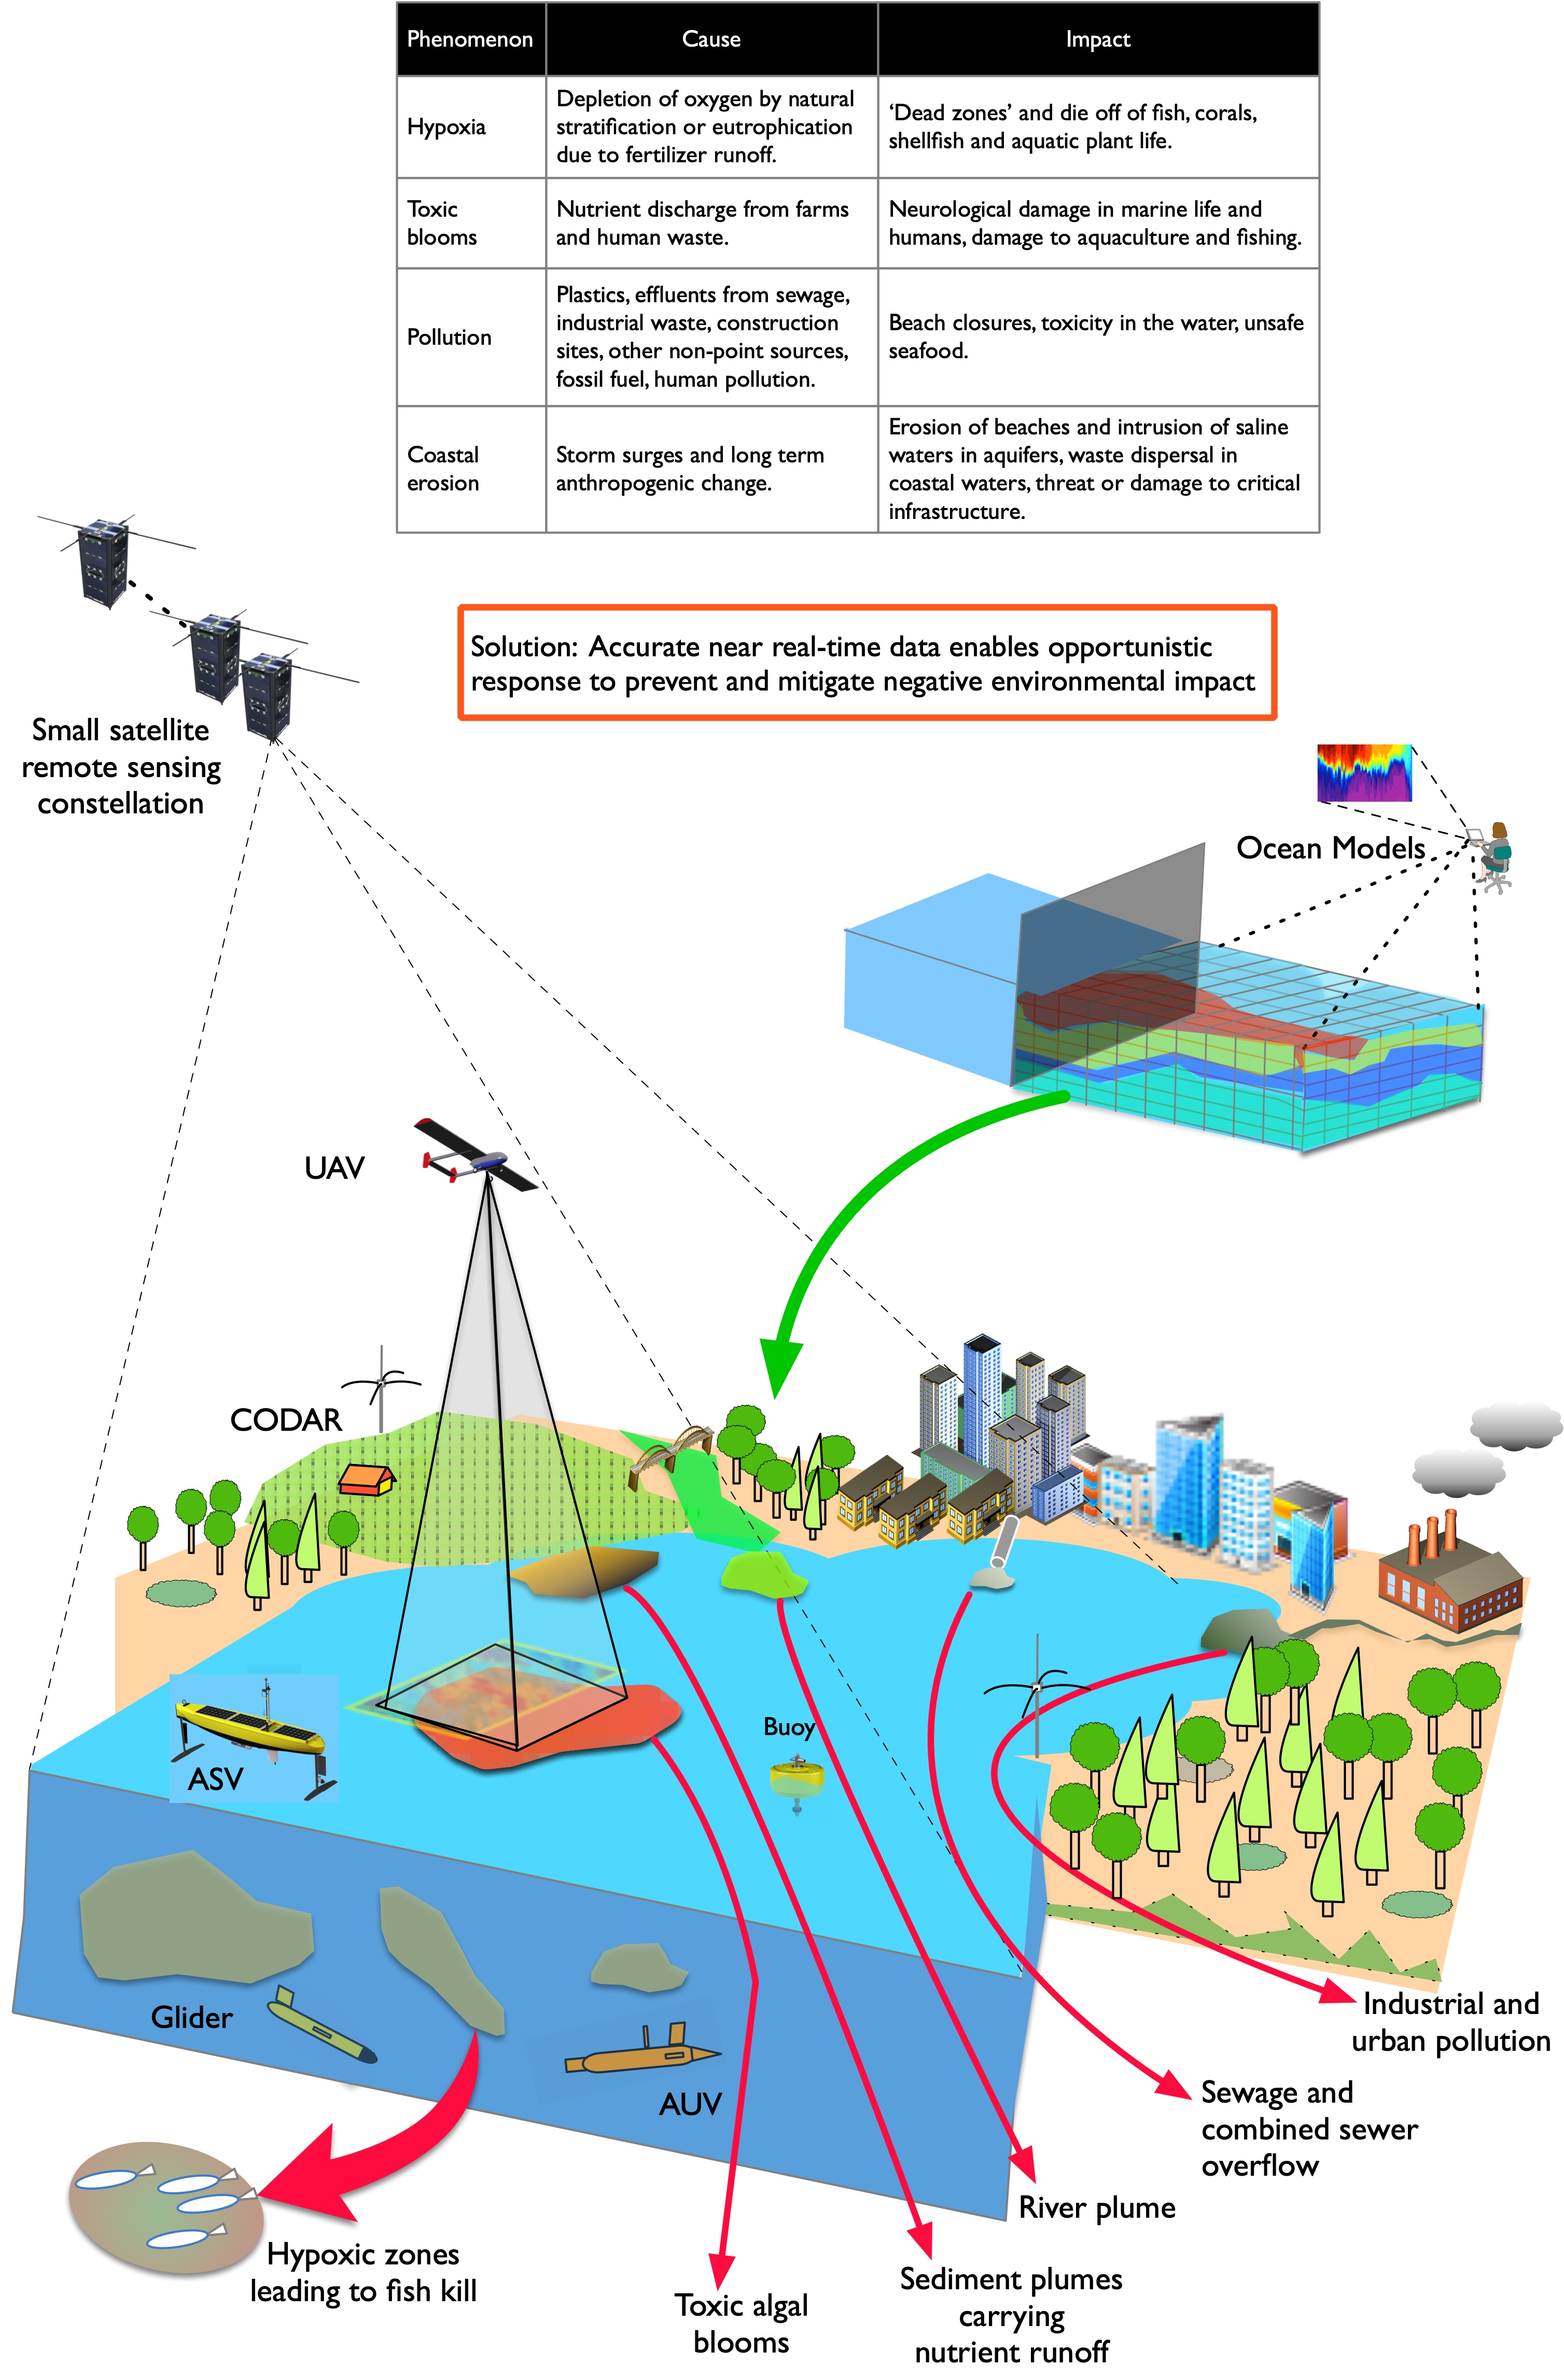
\includegraphics[scale=0.122]{fig/mega-cities-toxic-1.jpg}
  \caption{Coastal zones are impacted by human-induced activities
    leading to oxygen depleted hypoxic zones, toxic algal blooms,
    pollution, and coastal erosion. \pro will use an ensemble of small
    satellites, aerial, surface and underwater vehicles along with
    predictive shore-side ocean models, to observe the coastal ocean
    over sustained periods of time to provide real-time warning and
    situational awareness of impactful changes to human health,
    species diversity and ecosystem services. Note: UAV=Unmanned
    Aerial Vehicle; ASV=Autonomous Surface Vehicle; AUV=Autonomous
    Underwater Vehicle; CODAR=Coastal high-frequency radar.}
    \label{fig:mega-cities}
\end{figure}

\subsection{Why now?}

\begin{figure}[!t]
  \centering
  \includegraphics[scale=0.13]{fig/vehicles.jpg}
  \caption{Autonomous aerial and underwater vehicles from the Univ. of
    Porto, on a cruise in the Pacific in 2018.}
\label{fig:vehicles}
\end{figure}

With the onset of a climate crisis, the oceans are changing rapidly in
ways we do not understand.  In the report Global Marine Trends 2030,
Lloyds Register predicts that by 2030 the coastal ocean will be
“almost unrecognizable”. More than 800 million people, making up 10\%
of the earths population, live in urban centers along the coast -– the
“Urban Sea” -- and this Urban Sea supports their economic, nutritional
and recreational needs, as well as their well-being. Human induced
activities such as upstream fertilizer use for agriculture, industrial
activity, sewage discharge and urban combined stormwater overflow
cause the accumulation of pesticides, pollutants, pharmaceuticals, and
nutrients to end up in the Urban Sea.  In addition, climate change is
resulting in catastrophic damage to the coastal system.  Given the
urgency of meeting these threats, we cannot continue to study the
oceans and model their behavior the same way we have done before.

% There is an urgent need to develop and deploy
% new smart observational methods to provide information at scales that
% matter to the 600 million people living along the coast within 10
% meters of sea level.  Predicting change and providing early warning of
% hazardous events is essential for the well-being of an increasingly
% vulnerable coastal ecosystem and community. It is also in line with
% the goals of the 2021-2030 UN Decade of Ocean Science for Sustainable
% Development.


% The oceans cover more than 70\% of the earth's surface. The base of
% the human food-chain starts with tiny phytoplankton which generate the
% oxygen for every other breath we take.  With the onset of a climate
% crisis, the oceans are changing rapidly in ways we do not
% understand. There is an urgent need to develop and deploy new smart
% observational methods to provide information at scales that matter to
% the 600 million people living along the coast within 10 meters of the
% sea level.  Predicting change and providing early warning of hazardous
% events, including poor water quality, tainted fish stocks and
% intensifying coastal erosion, is essential for the well-being of an
% increasingly vulnerable coastal ecosystem. It is also in line with the
% goals of the 2021-2030 UN Decade of Ocean Science for Sustainable
% Development.

% By leveraging rapid advances in technology, \pro will field an
% innovative system of small satellites and robust autonomous in-situ
% platforms for obtaining unprecedented views of coastal oceans and
% atmospheric and land interfaces. It will aid in the understanding and
% monitoring of coastal waters so that they can be explored and utilized
% in a sustainable and informed manner.

% \pro will leap-frog the traditional incremental and siloed methods in
% ocean observation by leveraging modern computational methods in data
% science, autonomous robotics and smart sensors. The density and
% diversity of observations will change by an order of magnitude, the
% temporal scales of coastal observations will change from weeks (for
% traditional shipboard sampling) or days (for existing satellite data)
% to hours and minutes with the provision of real-time information.



\vspace*{-0.2cm}
\subsection{What is the novelty?}

Traditional  and  current  methods  for  observing  the  coastal
ocean  are  inefficient,  too sparse in space and sporadic in time, or
too localized. There is poor integration and assimilation of multiple
data sources - especially between those made in-situ and those made by
satellites - to produce actionable knowledge.

% \pro is different from traditional methods for observing the coastal
% ocean, which are inefficient, not cost-effective, too sparse in space,
% too sporadic in time or too localized. There is poor integration and
% assimilation of multiple data sources especially between those made
% in-situ and those made by satellites to produce actionable knowledge.

\pro is different as it leap-frogs current methods by delivering
advanced predictive modeling, Machine Learning and AI-driven
analytical capabilities, augmented by visualization techniques that
optimize observations but are non-existent in other interventions. The
density and diversity of observations will change by an order of
magnitude; the temporal scales of coastal observations will change
from weeks or days to hours and minutes with the provision of near
real-time information. Current remote sensing observations are
available at best once a day, while with a \sml constellation we can
provide a better quality data every 3 hours. Techniques in AI will
adapt the information for dissemination depending on the kind of user,
from well-informed scientists or government officials to the lay
person curious about how beach conditions might impact their
leisure.



The information will also be delivered via an app on a
smartphone or tablet and will be freely available for registered
users. % \color{blue} Advanced modeling
% predictions and analyses will be fully integrated with observations
% and learning, including real-time planning and autonomous adaptation
% to dynamical events and societal needs. \color{black}


% leap-frogs current methods by delivering predictive modeling,
% Machine Learning and AI driven analytical capabilities, augmented by
% visualization techniques that are non-existent in other interventions.
% The density and diversity of observations will change by an order of
% magnitude, the temporal scales of coastal observations will change
% from \emph{weeks or days} to \emph{hours and minutes} with the
% provision of near real-time information. Techniques in AI will adapt
% the information for dissemination depending on the kind of user, from
% well-informed scientists, government officials to the lay person
% curious about how beach conditions might impact her leisure.

% \pro leap-frogs current methods by delivering predictive modeling,
% Machine Learning and AI driven analytical capabilities, augmented by
% visualization techniques that are non-existent in other interventions.
% With \proe, the density and diversity of observations will change by
% an order of magnitude, the temporal scales of coastal observations
% will change from weeks (for traditional shipboard sampling) or days
% (for existing satellite data) to \emph{hours and minutes} with the
% provision of real-time information. Techniques in AI will adapt the
% information depending on the kind of user, from well-informed
% scientists, to the lay person curious about how beach conditions might
% impact her leisure.

% In the process of providing actionable knowledge, \pro will enable new
% modes of management and new understanding about coastal ocean
% processes in ways simply not possible before. \pro will allow citizens
% to develop critical understanding of the rapid change taking place in
% their Urban Seas and to ‘connect the dots’ between human activity and
% the effect on the environment around them. Citizen scientists will be
% engaged in generating new observations and be able to derive new
% knowledge about how ocean processes work. Scientists will be able to
% pose (and answer) new questions that could not have been asked
% before. And policy makers will have the tools to make informed
% decisions in time scales that matter, while developing truly
% integrative policies on ocean sustainability and
% stewardship.

% \pro will serve as a replicable blueprint for Ocean
% observation in targeting integration, synthesis, cost-effectiveness
% and scalability.


% In the process of providing actionable knowledge, \pro will enable new
% modes of management and new understanding about coastal ocean
% processes in ways simply not possible before.

In the process of providing actionable knowledge, \pro will enable new
modes of management and new understanding about coastal ocean
processes in ways simply not possible before.  While prototypes of
systems that combine remote sensing with ocean models exist, most of
these systems do not provide the kinds of near real-time information
at spatial scales (10s--100s of meters) relevant to coastal managers
or citizens.  \pro will overcome this challenge by combining
intelligently deployed in-situ sensors with high resolution
($\sim100$m) satellite data and assimilating ocean models to produce
layers of data of increasing complexity accessible to everyone from
citizens on the beach to scientists. \pro will allow citizens to
develop critical understanding of the rapid changes taking place in
their urban oceans/seas and to connect the dots between human activity
and the effect on the environment around them. Citizen scientists will
be engaged in generating new observations and be able to derive new
knowledge about how ocean processes work. Scientists will be able to
pose and address new questions that could not have been asked before,
and policymakers will have the tools to make informed decisions in
time scales that matter, while developing truly integrative policies
on ocean sustainability and stewardship.


% While some coastal ocean observatories use a limited number of robotic
% assets or remote sensing data, \pro is unique in the range and
% diversity of how these sensors are deployed, how data is integrated
% and synthesized, and how citizen engagement is used to improve the
% value of the output.  Additionally \pro provides an integrative
% open-source framework to connect robots, services and users in a
% seamless manner that is both scalable and replicable, providing a
% blueprint for other initiatives worldwide. It leap-frogs current
% methods by delivering 21st century predictive modeling, learning and
% analytical capabilities, which are supported by AI and visualization
% techniques that are non-existent in other interventions.

\subsection{Milestones and Deliverables}

\pro milestones and deliverables will be along the following lines:

% Overall expenses related to personnel and equipment for a 4 year term
% of project development, testing and initial deployment in
% \ref{fig:expense}. The overall proportion of the costs in
% \ref{fig:exp-pie}

% \begin{table}[!h]
%   \centering
%   \vspace{-0.5cm}
%   \begin{tabular}{|p{1.8cm}|p{13cm}|}\hline 
%     \rowcolor{Gray}
%     \bfseries Year &\bfseries Description \\
%     \hline
%     \textbf{Sept/Oct 2021} & Proof-of-concept field demonstration off of
%                              Portugal, with assimilation of measurements from aerial, surface and
%                              underwater vehicles into oceanographic models with remote sensing
%                              provided by a \nas \sml overflight and other sources.\\  
%     \hline
%     \textbf{1} & Architectural system design with a focus on software
%                  integration, building hardware and design and testing of Machine
%                  Learning for ocean model prediction.\\ 
%     \hline
%     \textbf{1--2} & Use and integration of existing remote sensing data products
%                     (from \esa and \nase), integration of ocean models and building of
%                     AI-based adaptive control systems for aerial, surface and underwater
%                     vehicles. \\  
%     \hline
%     \textbf{1--2} & Incremental demonstration of closing the
%                     prediction-sensing-assimilation loop for dynamic ocean events in the
%                     coastal region.\\
%     \hline
%     \textbf{1--3} & Incremental at-sea testing of adaptations of robotic vehicles
%                     and integration of control with ocean model predictions.\\

%     \hline
%     \textbf{1--3} & Demonstrations of the integrative software system using existing
%                     aerial, surface and underwater vehicles and targeting a single
%                     use-case (e.g. from aquaculture, oil \& gas, others) for
%                     monetization.\\
%     \hline
%     \textbf{3--4} & Upscope demonstration to include larger data sources for
%                     physical ocean properties, including
%                     from buoys and surf forecasts.\\ 

%     \hline
%     \textbf{3--4} & Pursue European Union and other sources to fund a constellation
%                     of \smle's to demonstrate the full capability in a coastal ecosystem.\\ 
%     \hline
%   \end{tabular}
%   \caption{Proposed timeline of milestones and deliverables.}
%   \label{tab:timeline}
%   \vspace{-0.5cm}
% \end{table}

\ifkeck

\begin{itemize}[noitemsep,topsep=0pt,parsep=5pt,partopsep=10pt]

\item Architectural system design with a focus on software
  integration (Year \textbf{1})

\item HOPS modeling customized for targeted coastal domain (US
  east-coast) (Year \textbf{1})

\item Use and integration of existing remote sensing data products
  (from \esa and \nase), integration of ocean models and building of
  AI-based adaptive control systems for aerial, surface and underwater
  vehicles.  (Years \textbf{1})

\item Design of automated data pipeline for quality-controlled data
  assimilation from a range of sources (Year \textbf{1})

\item Design and testing of Machine Learning for ocean model
  prediction and convergence (Year \textbf{1--2})

\item Design, test and implementation of sampling algorithms for
  embedded reasoning (Year \textbf{1--2})

\item Phased demonstration of closing the
  prediction-sensing-assimilation loop for dynamic ocean events in the
  coastal region (Years \textbf{2})

\item Phased at-sea testing of adaptations of robotic vehicles and
  integration of control with ocean model predictions (Years
  \textbf{1--2})

% \item Demonstrations of the integrative software system using existing
%   aerial, surface and underwater vehicles and targeting a single
%   use-case (e.g. from aquaculture, oil \& gas, coastal pollution
%   around urban centers, others) for monetization (Year \textbf{1--3})

% \item Upscope demonstration to include larger data sources for
%   physical ocean properties, including from buoys and surf forecasts
%   (Years \textbf{3--4})

% \item \sml launch and operation begins. Validation of satellite
%   payloads and calibration of sensor performance (Years \textbf{4--5})

% \item Pursue other sources to fund a constellation
%   of \smle s to demonstrate the full capability in a coastal ecosystem
%   (Years \textbf{3--4})
  
\end{itemize}

\else

\begin{itemize}[noitemsep,topsep=0pt,parsep=5pt,partopsep=10pt]

\item A Sept/Oct 2021 proof-of-concept field demonstration off of
  Portugal, with assimilation of measurements from aerial, surface and
  underwater vehicles into oceanographic models with remote sensing
  provided by a cubesat that was developed with funding from the Moore
  Foundation as well as other more traditional sources.

\item Architectural system design with a focus on software
  integration, building hardware and design and testing of Machine
  Learning for ocean model prediction (Year \textbf{1})

\item Use and integration of existing remote sensing data products
  (from \esa and \nase), integration of ocean models and building of
  AI-based adaptive control systems for aerial, surface and underwater
  vehicles.  (Years \textbf{1--2})

\item Phased demonstration of closing the
  prediction-sensing-assimilation loop for dynamic ocean events in the
  coastal region (Years \textbf{1--2})

\item Phased at-sea testing of adaptations of robotic vehicles and
  integration of control with ocean model predictions (Years
  \textbf{1--3})

\item Demonstrations of the integrative software system using existing
  aerial, surface and underwater vehicles and targeting a single
  use-case (e.g. from aquaculture, oil \& gas, coastal pollution
  around urban centers, others) for monetization (Year \textbf{1--3})

\item Upscope demonstration to include larger data sources for
  physical ocean properties, including from buoys and surf forecasts
  (Years \textbf{3--4})

% \item \sml launch and operation begins. Validation of satellite
%   payloads and calibration of sensor performance (Years \textbf{4--5})

\item Pursue European Union and other sources to fund a constellation
  of \smle s to demonstrate the full capability in a coastal ecosystem
  (Years \textbf{3--4})
  
\end{itemize}

\fi

\ifkeck
\begin{figure}[!t]
  \centering
  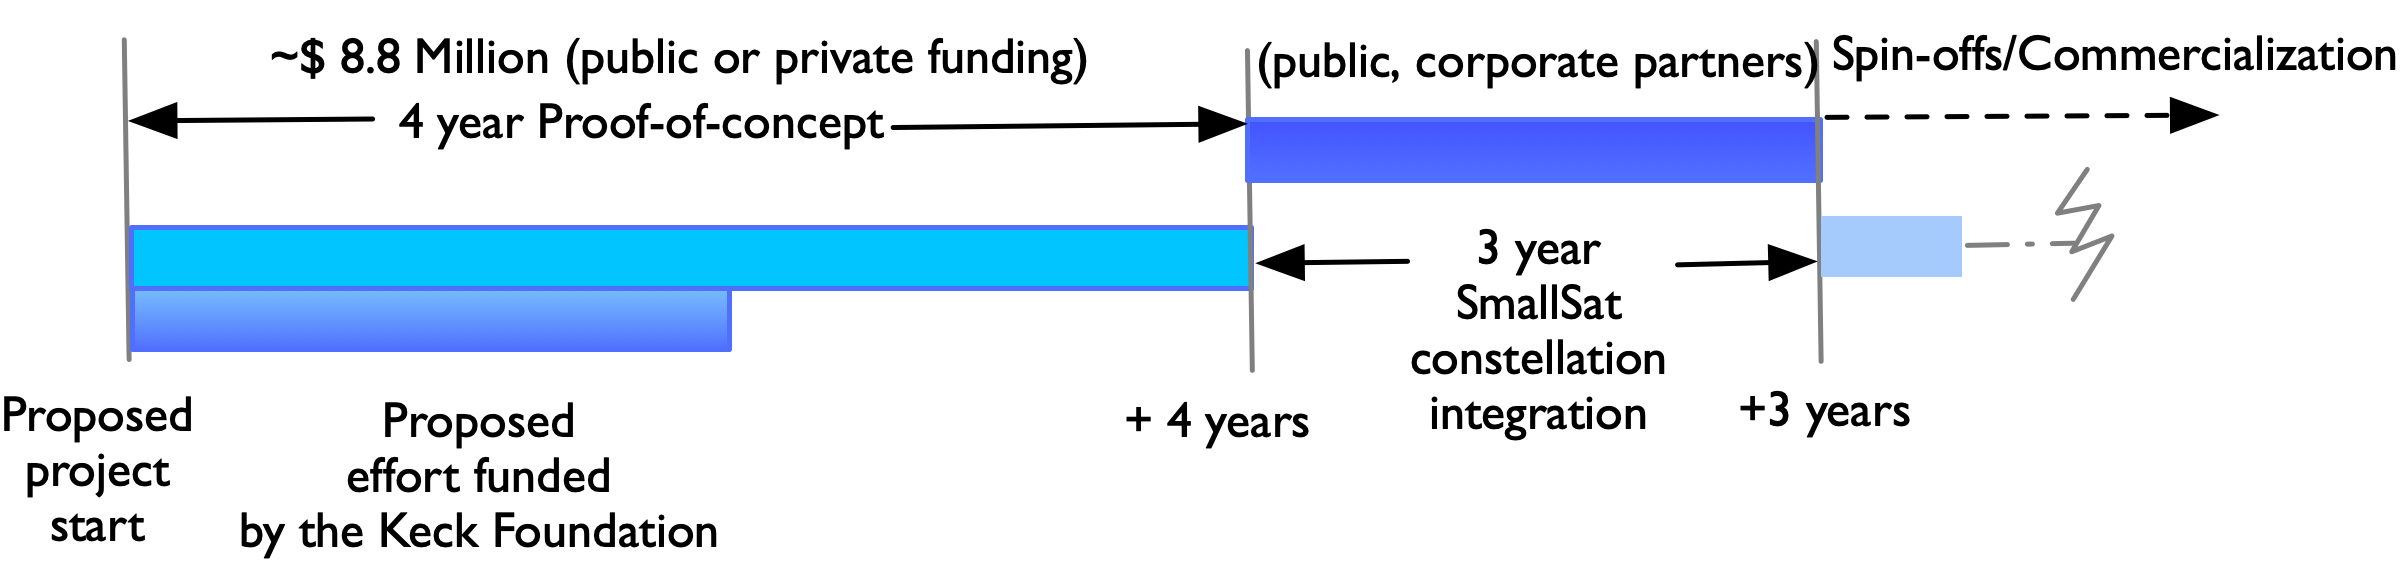
\includegraphics[scale=0.19]{fig/timeline-keck.jpg}
  \caption{Overview of timeline in steps for \proe. Support from the
    \kck would build the foundations for modeling and sampling
    followed by a other funding to ensure a systematic engineering
    effort to build the needed software infrastructure. Should \sml
    constellation build/test/launch/flight and purchase of hardware be
    possible, that effort can be accommodated with the software build
    shown.}
  \label{fig:timeline}
\end{figure}

\else

\begin{figure}[!t]
  \centering
  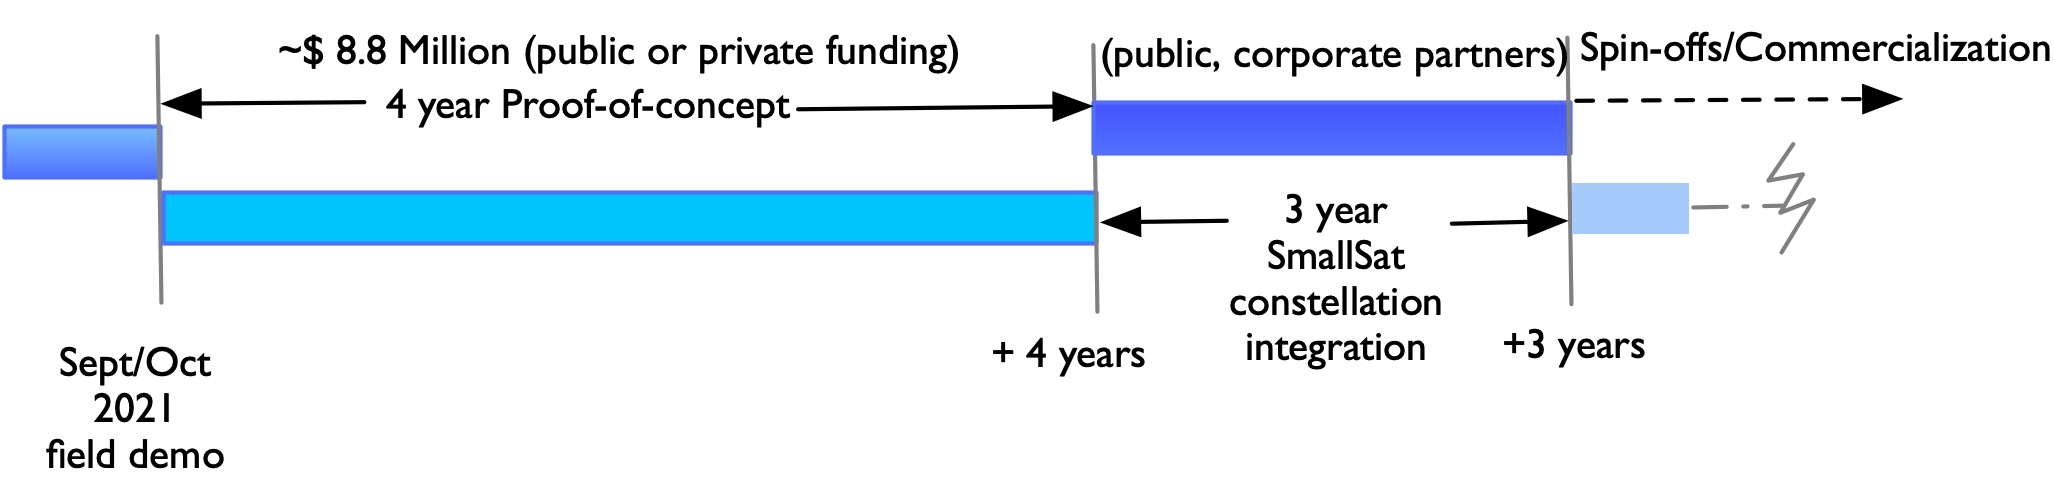
\includegraphics[scale=0.22]{fig/timeline.jpg}
  \caption{Overview of timeline in steps for \proe. Initial
    demonstration of key concepts with a simple demonstration in a
    field experiment in 2021 would ideally be followed by a systematic
    engineering effort to build the needed software
    infrastructure. Should \sml constellation build/test/launch/flight
    and purchase of hardware be possible, that effort can be
    accommodated with the software build shown.}
  \label{fig:timeline}
\end{figure}

\fi

\ifkeck
\else
% \noindent
Our first step will be a rapid and simple demonstration of the key
concepts in the September/October 2021 timeframe using existing remote
sensing products including that from an ocean color cubesat funded by
the Moore Foundation for environmental assimilation, and available
robotic platforms, for an experiment that links in-situ measurements
with ocean model assimilation, prediction and intelligent adaptive
sampling. We will use this exercise to demonstrate to key stakeholders
the potential of systematic integration of platforms and sensors, with
models, so as to visualize in detail, generated data products. A more
systematic integration, the focus of this proposal, will require the 4
year effort proposed above. Should sponsorship of the \sml
constellation occur during this phase, the build/test/launch/flight
and integration of these assets with the software will
commence. Subsequent spin-offs and commercialization will need skilled
staff to do the outreach to a range of commercial, governmental and
NGO entities.
\fi

% \begin{wrapfigure}{r}{0.45\textwidth}
%   % \vspace{-1cm}
%   \centering
%   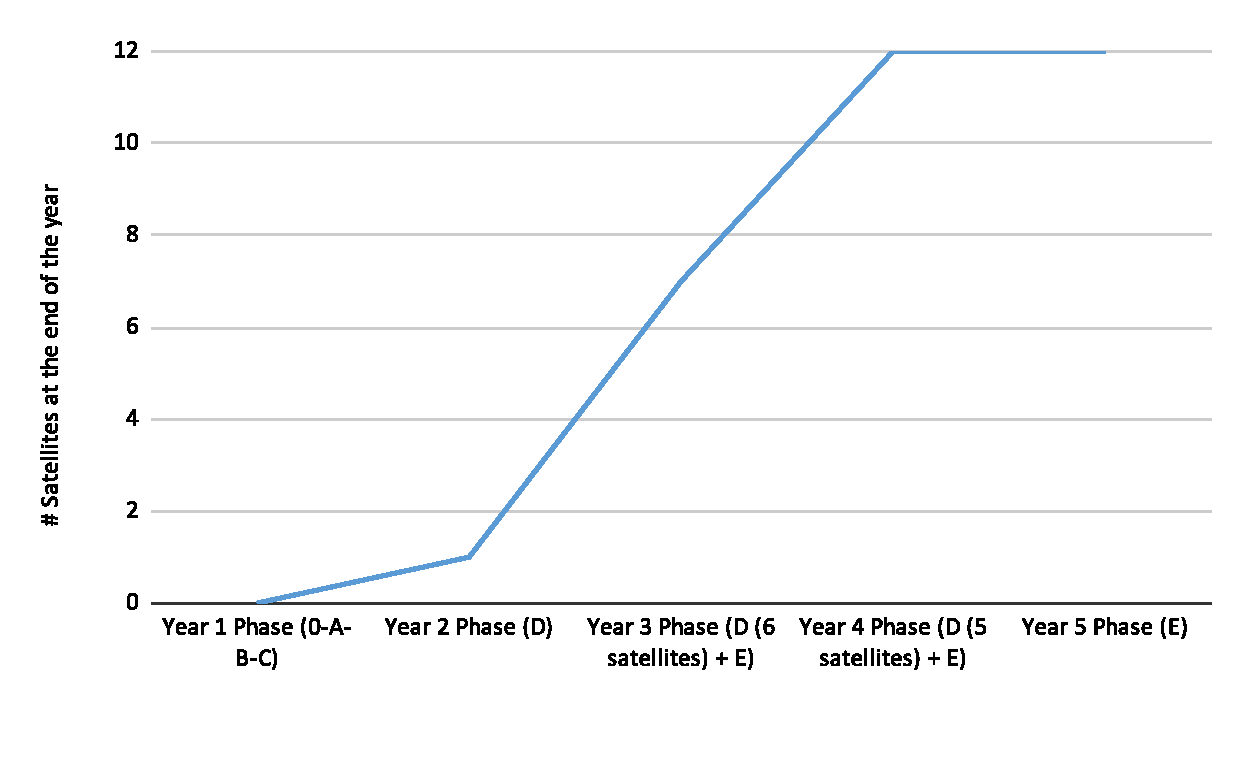
\includegraphics[scale=0.35]{fig/sat-progression.pdf}
%   \caption{Progression of deployment for 12 \smle's over a period of 5
%     years.}
%   \label{fig:sat-prog}
%   % \vspace{-0.5cm}
% \end{wrapfigure}


% shows costs associated with the project broken
% down to provide a clear picture of the distributions of proposed
% expenses. The end product will be a software system which will predict
% oceanographic conditions, use the prediction to adaptively place
% in-situ robotic vehicles to sample at the 'right place and right
% time', assimilate the sensed environment in ocean models and provide a
% reiterated prediction.

% Should the \sml part of the project be simultaneously
% executed with the development of software and hardware for in-situ
% assets, the two figures would then be merged. The incremental
% deployment of the \smle's is shown in Fig. \ref{fig:sat-prog}.

% \parbox[t]{\dimexpr\textwidth-\leftmargin}{%
%       \vspace{-2.5mm}
%       \begin{wrapfigure}[10]{r}{0.5\textwidth}
%         \centering
%         \vspace{-\baselineskip}
%         \subfigure[]{\label{fig:insitu}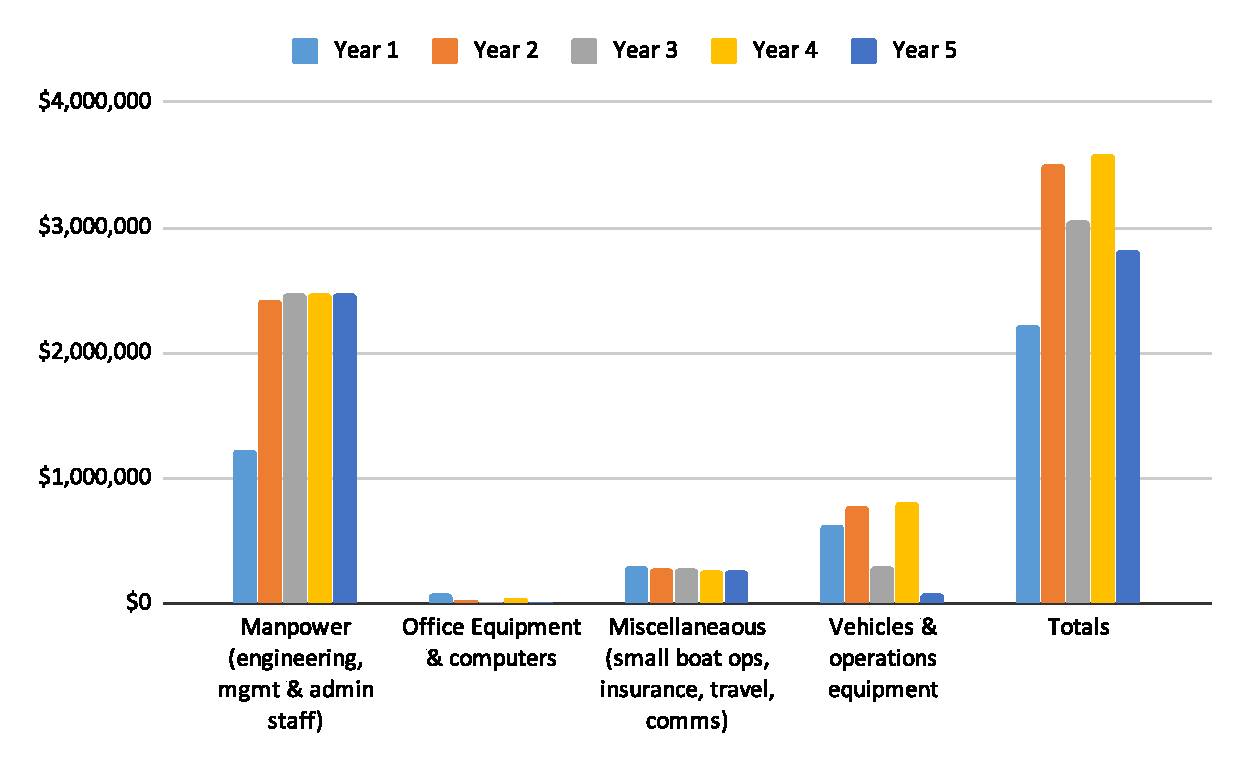
\includegraphics[width=.75\linewidth]{fig/insitu.pdf}}
%         \subfigure[]{\label{fig:sats}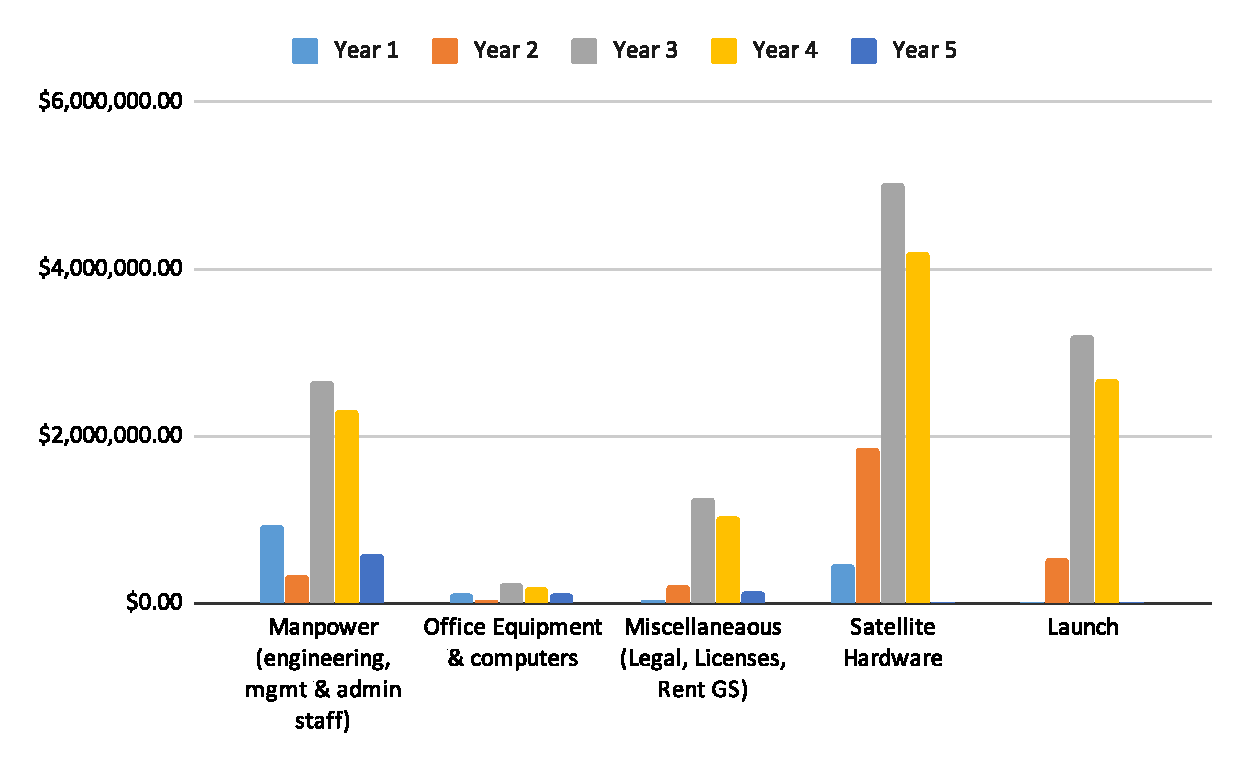
\includegraphics[width=.75\linewidth]{fig/sats.pdf}}
%         \caption{Costs and distribution for \ref{fig:insitu} assets and
%           software and \ref{fig:sats} \smle's over a 5 year project term.}
%       \end{wrapfigure}
%     }

% \noindent
Fig. \ref{fig:timeline} shows the overall timeline associated with the
\pro project.  Fig. \ref{fig:costs} shows the anticipated cost
breakdown to provide a clear picture of the distribution of the
budget. The end product will be a software system that will predict
oceanographic conditions, use the prediction to adaptively place
in-situ robotic vehicles to take water samples at the ‘right place and
right time’, assimilate the sensed environment in ocean models and
provide a reiterated prediction.

\begin{figure}[!h]
  \centering
  \subfigure[]{\label{fig:expense}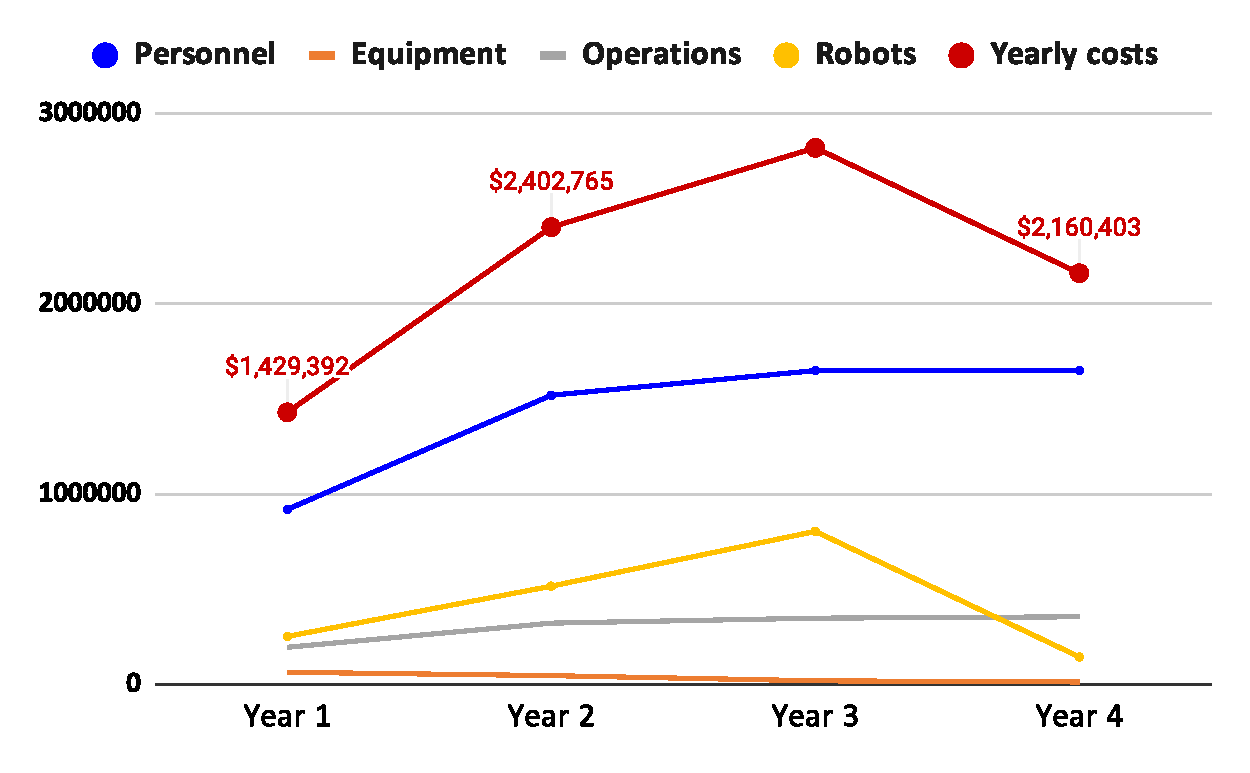
\includegraphics[scale=0.4]{fig/expenses.pdf}}
  \subfigure[]{\label{fig:exp-pie}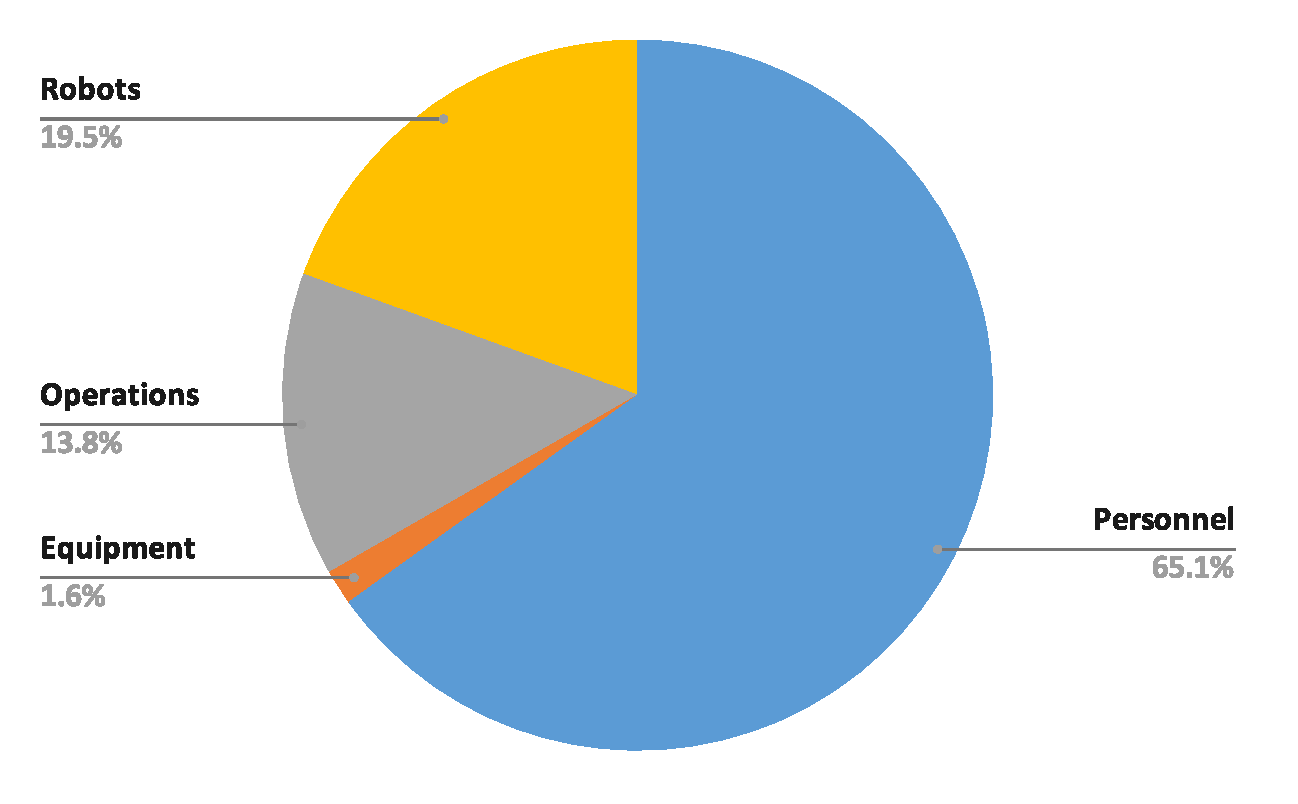
\includegraphics[scale=0.36]{fig/expenses-pie.pdf}}
  \caption{Budget needs and distribution for a 4-year project term:
    \subref{fig:expense} Total expenses related to personnel and
    equipment for a 4-year term; \subref{fig:exp-pie} Proportions of
    total budget for different uses (4-year averages).}
  \label{fig:costs}
  \vspace{-0.5cm}
\end{figure}

\subsection{Resources Needed}

The \pro team (see biographies below) comes ready with aerial, surface
and underwater vehicle platforms, together with the extensive suite of
communication software to provide coordinated observations in the
coastal ocean at the UPorto and SOCIB. With sensors measuring key
ocean variables, the focus of our effort will be in integrating
multiple data streams, increasing modeling skill with assimilated data
and adaptively targeting the in-situ vehicles to narrow the knowledge
gap of current oceanographic conditions. For this effort we will
continue to rely on existing remote sensing data products for
environmental assimilation. This in turn will provide a clear
consistent set of data products to provide actionable information to
policymakers on the ground, and society at large.

% comes ready with aerial, surface and underwater vehicle platforms,
% together with the extensive suite of communication software to provide
% coordinated observations in the coastal ocean at the \univ and
% \soce. With sensors measuring key ocean variables, the focus of our
% effort will be in integrating multiple data streams, increasing
% modelling skill with assimilated data and adaptively targeting the
% in-situ vehicles to narrow the knowledge gap of current oceanographic
% conditions. For this effort we will continue to rely on existing
% remote sensing data products for environmental assimilation. This in
% turn
% % We will integrate custom sensors keyed towards important ocean
% % variables integrated into a 'train' of \sml platforms.  Such a system
% % working synchronously with in-situ robots
% will provide a clear consistent set of data products to provide
% actionable information to policymakers on the ground, as also society
% in general.

We estimate the total project cost to be $\sim\$8.8$ Million over a
period of 4 years. As milestones are met in the first two years, and
the integrated software can be demonstrated on targeted use-cases,
\pro is likely to attract funding from public and private
sources. % Consequently, the project can also be funded in incremental
% steps:

% \begin{itemize}[noitemsep,topsep=0pt,parsep=0pt,partopsep=0pt]

% \item an initial focus on the software build, integration and test
%   with available robotic vehicles in small scale demonstrations $\sim
%   \$5$--$\$10$ Million for years 1 \& 2.

% \item acquisition of robotic vehicles, buoys, floats and a range of
%   sensors as payloads for these in-situ vehicles, their integration,
%   deployment and demonstration at increasingly larger spatial and
%   temporal scales for $\sim \$20$--$\$30$ Million in years 2 \& 3.

% \item acquisition of funds for a suitable at-scale design, build,
%   test, launch and operation of a \sml constellation with a range of
%   scientific payloads for biological and physical oceanographic
%   measurements for $\sim \$25$ Million in years 4 \& 5.

% \end{itemize}  

% Incremental build and evaluation of this concept can allow us to
% attract a wide range of public and private sponsors in the US and
% Europe.  Equally, we will consistently work with our collaborators in
% the Portuguese government to leverage expensive ship time for testing,
% and other potential in-kind contributions from Portuguese and Spanish
% resources.

% For a long-term operation and viability of this system, multiple
% outcomes can be envisioned. First, with the experience garnered in
% testing and fielding the system, a commercial spin-off of all or parts
% of the technology could be likely. If parts of the technology could be
% monetized and spun off to other companies, \pro can then hold the IP
% while continuing to work on research outcomes after the 4 year
% term. Second, the project can itself look for contracts from
% mega-cities and governments or their agencies to provide a
% software-as-a-service model and be able to subsist as a not-for-profit
% enterprise with unique expertise. Should other private or public
% funding sources be available, those would also be carefully evaluated
% to sustain operations and maintain an R\&D effort.

For a long-term operation and viability of this system, multiple
outcomes can be envisioned. First, with the experience garnered in
testing and fielding the system, a commercial spin-off of all or parts
of the technology could be likely. If parts of the technology could be
monetized and spun off to other companies, \pro can then hold the IP
while continuing to work on research outcomes after the 4-year
term. Second, the non-profit entity that will run the project, can
itself look for contracts from mega-cities and governments or their
agencies to provide a software-as-a-service model and be able to
subsist as a not-for-profit enterprise with unique expertise. Should
other private or public funding sources be available, those would also
be carefully evaluated to sustain operations and maintain an R\&D
effort.


\subsection{Governance and Execution}


The governing board of \pro will consist of prominent strategic
advisors from the US and Europe including stakeholders and funders. In
addition, the project principals will be aided and advised by a
scientific advisory board consisting of technologists, ocean-going
scientists, ecologists and policymakers from the US, Europe and
targeted coastal states.

The project itself will be based in Porto, Portugal, with support from
all team partners, for a number of important reasons including the
existence of marine robotic development and testing infrastructure, a
skilled tech-savvy work force, university support and overall
cost-effectiveness.  % \color{blue} Of course, the team will also
% involve their respective facilities.  In the last two years, to
% demonstrate portability and rapid responses to regional events,
% additional centers will be created in Spain and east and west coasts
% of the US.  \color{black}

% \newpage
\subsection{The Team}

\proe’s interdisciplinary team of seasoned researchers from the US
(\orge, Columbia University and MIT), Portugal and Spain have worked
in all the major oceans, fielded tens of robots at sea simultaneously,
designed/built/flown and operated multiple \smle s and complex systems
in the deep ocean and deep space. Hence they have a proven track
record of theoretical and practical understanding of the work that
needs to be accomplished individually and collaboratively. They have
also worked extensively with each other, which optimizes the chances
for effective team effort needed by this project to succeed.

% inter-disciplinary team of seasoned researchers (see bio's
% below) from the US (\org, Columbia and MIT), Portugal and Spain have
% worked in all the major oceans, fielded tens of robots at sea
% simultaneously, designed/built/flown and operated multiple \smle's and
% complex systems in the deep sea and deep space. They have also worked
% extensively with one another.
